%
\documentclass[11pt]{thesis} % draft

\title{Algorithmic Meta-Creativity}
\author{Fania Raczinski}
\date{March 2015}

% Test

\begin{document}

\subsubsection{Manipulation}

Within the manipluation category, (different representations of) sounds are pataphysicalised directly. There are several approaches to this, such as making changes to sound wave forms (an antinomy pataphysicalisation for example could be to invert a sound wave, i.e. where there was silence there is now noise and vice versa). These manipulations could be applied to specific sections only or the complete sound wave. This kind of manipluation could also be applied to musical scores. Changes might also happen in given compositions of music of multiple instruments (as opposed to pataphysicalising the composition process itself which is covered in section~\ref{s:composition}\marginpar{§~\ref{s:composition}}).

\begin{figure}[!htbp]
\centering
  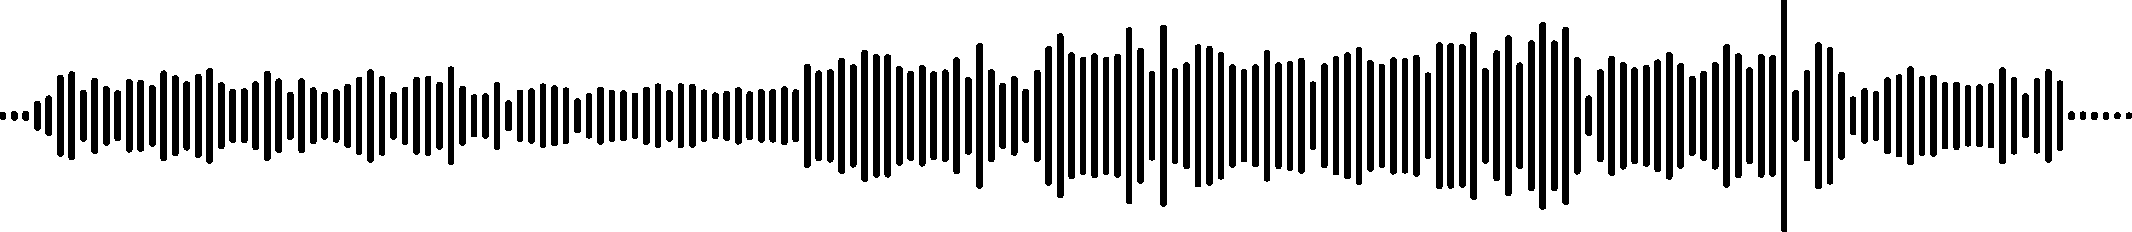
\includegraphics[width=\linewidth]{simplewave.pdf}
\caption[Sound wave of \textit{La Chanson Du D{\'e}cervelage}]{Sound wave of \textit{La Chanson Du D{\'e}cervelage} \autocite[][Track 1]{UbuWebPata} (generated using \autocite{Heesakkersnd})}
\end{figure}

Various tools might be useful for these sorts of manipulations, including the \textit{Web Audio API} by the \ac{W3C} \autocite{Adenot2017}. It includes ``capabilities found in modern game audio engines as well as some of the mixing, processing, and filtering tasks that are found in modern desktop audio production applications'' \autocite*{Adenot2017}. An example of using this API to synthesise sounds is described in \autocite{Misuary2016}. Other \ac{API}s such as SoundCloud \autocite{soundcloud} might be helpful as well. 

Another approach altogether could be to play with \ac{MIDI} \autocite{midind} but this needs to be explored a lot further.


\subsubsection{Search}

Similar to the image and video search of \url{pata.physics.wtf}, audio search could be based on tags provided through an \ac{API} such as FreeSound \autocite{freesoundnd}. 

\begin{quotation}
  The query does a weighted search over some sound properties including sound tags, the sound name, its description, pack name and the sound id. Therefore, searching for query=123 will find you sounds with id 1234, sounds that have 1234 in the description, in the tags, etc. \sourceatright{\autocite{freesoundnd}}
\end{quotation}

The search would work in a similar way then. Section~\ref{s:imgvid}\marginpar{§~\ref{s:imgvid}} specifies that we (1) translate query, (2) pataphysicalise the translation, and (3) retrieve matching images/videos using \ac{API} calls.

So, say the user query is `rumbling', that would be translated to `grondant' (French for `growling') and `\begin{CJK}{UTF8}{min}お叱り\end{CJK}' (Japanese for `scold') and finally the English `scolding'. From this we then produce a list of 10 patadata (`[berate, chide, call on the carpet, chiding, rag, lambast, bawl out, tongue-lashing, grouch, scold]') by pataphysicalising this translated term. This patadata is then used to actually retrieve sound files through an \ac{API}.

Issues that can arise with the use of external \ac{API}s and folksonomy (user generated tags) have already been mentioned in section~\ref{s:apis} and~\ref{s:imgalgoimprovs}\marginpar{§~\ref{s:apis}}. With sound files specifically perhaps tags might be very subjective. This may or may not be useful in a pataphysical context of course.


\subsubsection{Composition}
\label{s:composition}

- pata constraints to composition



\end{document}
